PageRank is an algorithm developed by Page and Brin \cite{rank-page99} for ranking web pages in search engine results, and is a key component of Google's search algorithm. It assigns a numerical score to each page, and is based on the principle that a page is important if it is linked to by other important pages. While PageRank was originally designed for web page ranking, it has broader applications in information retrieval, recommendation systems, predicting traffic flow, protein target identification, and fraud detection.

The proliferation of vast datasets represented as graphs has spurred significant interest in algorithms addressing graph-related challenges. With the increasing size and dynamism of networks, the demand for faster PageRank computation, especially on massive dynamic networks, has prompted the development of new algorithms and approaches. Researchers are actively exploring parallel and distributed algorithms, considering the challenges posed by shared-memory systems, including contention, false sharing, and memory access delays. The pursuit of faster and more efficient PageRank computation aligns with the imperative in the realm of big data analytics, where processing large datasets swiftly is of paramount importance.

As PageRank gains popularity, a wealth of research focuses on designing parallel algorithms for its computation. Various platforms such as multicore CPUs \cite{rank-garg16}, GPUs \cite{rapids}, FPGAs \cite{rank-guoqiang20}, SpMV ASICs \cite{rank-sadi18}, CPU-GPU hybrids \cite{rank-giri20}, CPU-FPGA hybrids \cite{rank-li21}, and distributed systems \cite{rank-sarma13} have been explored, employing techniques like power iterations, random walks, and Markov chains.

Despite these advancements, a crucial challenge arises in the context of dynamic graphs. In dynamic scenarios, graphs evolve through vertex and edge insertions and deletions, making it impractical to recompute PageRank entirely for small changes. Addressing this issue, Banerjee et al. \cite{rank-sahu22} investigate parallel dynamic algorithms for PageRank, leveraging techniques developed by Garg et al. \cite{rank-garg16}.

In this report, we present our contributions, adapting the "Barrier-free" PageRank to dynamic algorithms such as "Naive-dynamic" (\NaiBarf{}) and "Dynamic Traversal" (\TraBarf{}) in Sections \ref{sec:about-naive} and \ref{sec:traversal}. However, our evaluation indicates that \TraBarf{} falls short in performance.




\subsection{Our Contributions}

% We introduce the "Dynamic Frontier" approach in Section \ref{sec:frontier}, which identifies vertices likely to undergo rank changes with minimal overhead during batch updates.
This report introduces DF-PageRank\footnote{https://github.com/puzzlef/pagerank-openmp-dynamic}, an parallel shared-memory implementation of our Dynamic Frontier approach for updating PageRank scores on dynamic graphs. Our Dynamic Frontier approach incrementally identifies vertices likely to undergo rank changes with minimal overhead during batch updates. On a machine with two 16-core Intel Xeon Gold 6226R processors, GVE-Leiden achieves a processing rate of $352 M$ edges/s on a $3.8 B$ edge graph, and outperforms the original Leiden implementation, igraph Leiden, and NetworKit Leiden by $373\times$, $86\times$, and $7.2\times$ respectively, while identifying communities of the same quality as the first two implementations, and $26\%$ higher quality than NetworKit. Compared to GVE-Louvain, our parallel Louvain implementation, GVE-Leiden achieves an $11$-fold reduction in internally-disconnected communities, with only a $36\%$ increase in computation time. With doubling of threads, GVE-Leiden exhibits an average performance scaling of $1.6\times$.\ignore{This makes GVE-Leiden an attractive choice for high-quality community detection on massive graphs.}




%% - Use --- for a dash.
%% - Use ``camera-ready'' for quotes.
%% - Use {\itshape very} or \textit{very} for italicized text.
%% - Use \verb|acmart| or {\verb|acmart|} for mono-spaced text.
%% - Use \url{https://capitalizemytitle.com/} for URLs.
%% - Use {\bfseries Do not modify this document.} for important boldface details.
%% - Use \ref{fig:name} for referencing.

%% For a block of pre-formatted text: 
% \begin{verbatim}
%   \renewcommand{\shortauthors}{McCartney, et al.}
% \end{verbatim}

%% For a list of items:
% \begin{itemize}
% \item the ``ACM Reference Format'' text on the first page.
% \item the ``rights management'' text on the first page.
% \item the conference information in the page header(s).
% \end{itemize}

%% For a table:
% \begin{table}
%   \caption{Frequency of Special Characters}
%   \label{tab:freq}
%   \begin{tabular}{ccl}
%     \toprule
%     Non-English or Math&Frequency&Comments\\
%     \midrule
%     \O & 1 in 1,000& For Swedish names\\
%     $\pi$ & 1 in 5& Common in math\\
%     \$ & 4 in 5 & Used in business\\
%     $\Psi^2_1$ & 1 in 40,000& Unexplained usage\\
%   \bottomrule
% \end{tabular}
% \end{table}

%% For a full-width table:
% \begin{table*}
%   \caption{Some Typical Commands}
%   \label{tab:commands}
%   \begin{tabular}{ccl}
%     \toprule
%     Command &A Number & Comments\\
%     \midrule
%     \texttt{{\char'134}author} & 100& Author \\
%     \texttt{{\char'134}table}& 300 & For tables\\
%     \texttt{{\char'134}table*}& 400& For wider tables\\
%     \bottomrule
%   \end{tabular}
% \end{table*}


%% For inline math:
% \begin{math}
%   \lim_{n\rightarrow \infty}x=0
% \end{math},

%% For a numbered equation:
% \begin{equation}
%   \lim_{n\rightarrow \infty}x=0
% \end{equation}

%% For an unnumbered equation:
% \begin{displaymath}
%   \sum_{i=0}^{\infty} x + 1
% \end{displaymath}

%% For a figure:
% \begin{figure}[h]
%   \centering
%   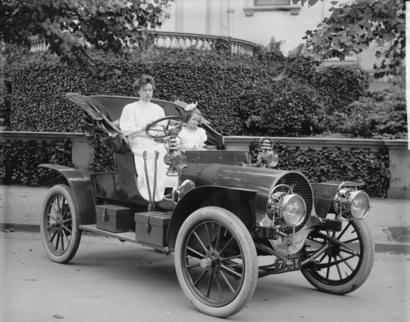
\includegraphics[width=\linewidth]{inc/sample-franklin}
%   \caption{1907 Franklin Model D roadster. Photograph by Harris \&
%     Ewing, Inc. [Public domain], via Wikimedia
%     Commons. (\url{https://goo.gl/VLCRBB}).}
%   \Description{A woman and a girl in white dresses sit in an open car.}
% \end{figure}

%% For a teaser figure.
% \begin{teaserfigure}
%   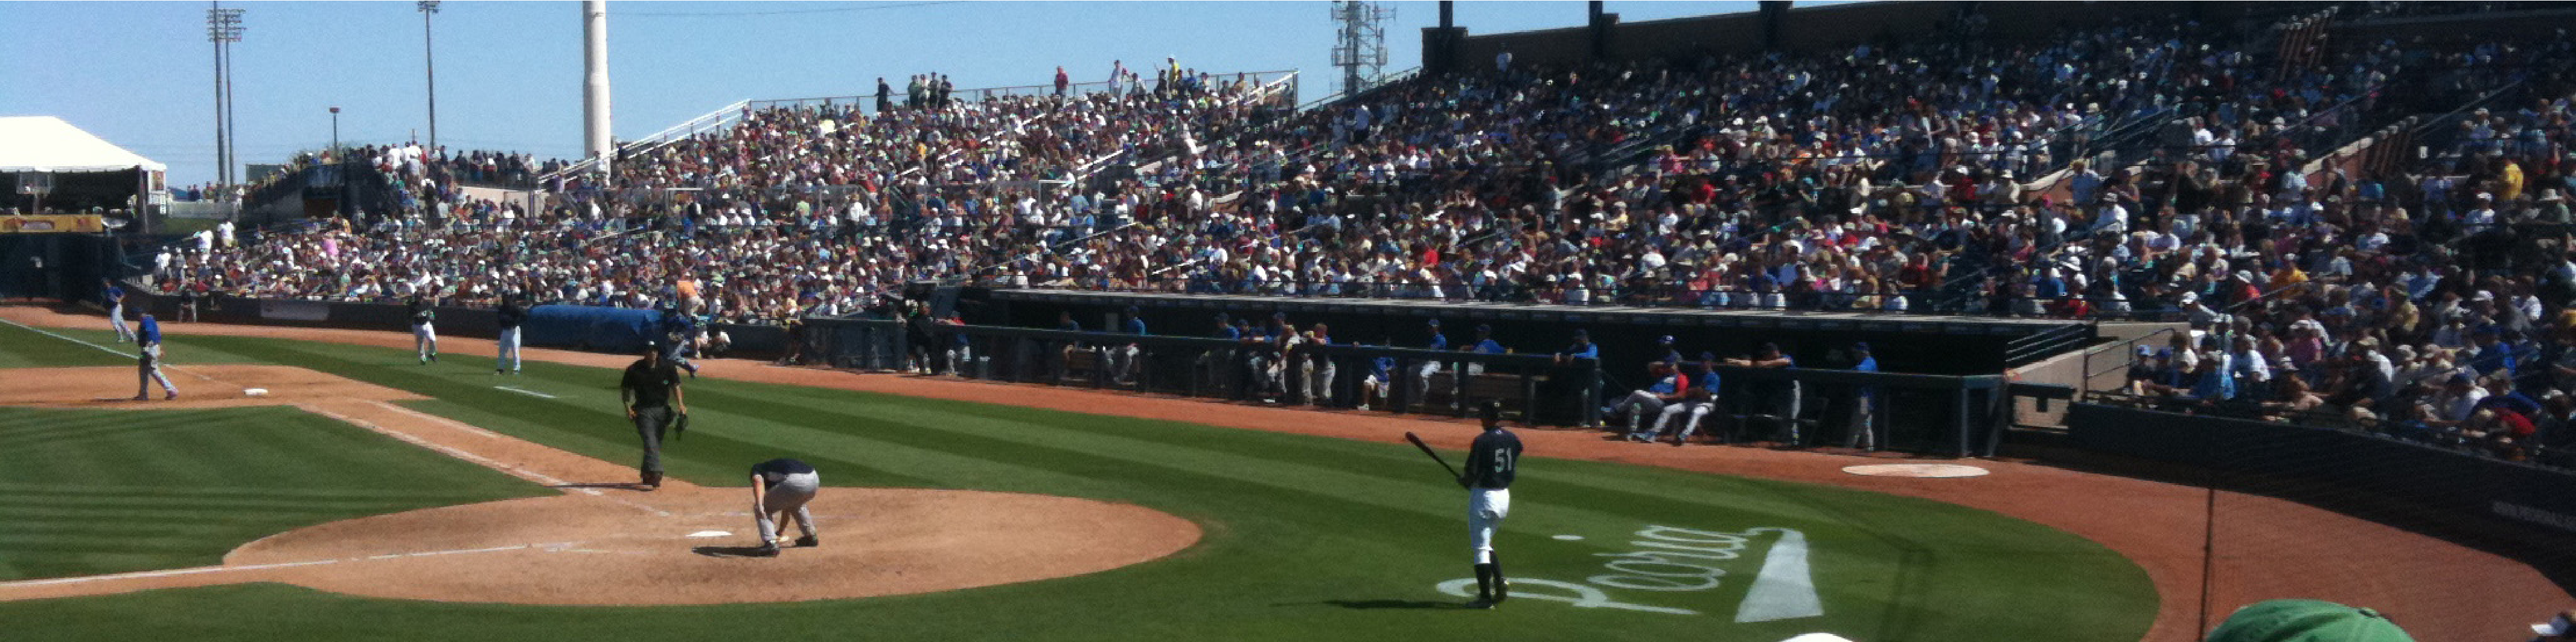
\includegraphics[width=\textwidth]{sampleteaser}
%   \caption{figure caption}
%   \Description{figure description}
% \end{teaserfigure}
